%# -*- coding: utf-8 -*-
% !TeX encoding = UTF-8 Unicode
% !TeX spellcheck = en_US
% !TeX TS-program = xelatex
%~ \XeTeXinputencoding "UTF-8"
% vim:ts=4:sw=4
%
% 以上设定默认使用 XeLaTex 编译,并指定 Unicode 编码,供 TeXShop 自动识别

\chapter{app-ns2}

\section{High Level Design}



\begin{enumerate}
  \item 使用 flowchart 将处理流程初步理清
  \item 使用 \href{http://www.cascading.org/}{Cascading}/MapReduce 实现系统
  \item 测试
\end{enumerate}


\subsection{介绍}

\begin{enumerate}
  \item simulation task:
  generate the NS2 TCL scripts, and run ns2

  \item plotting figures:
  
\end{enumerate}


\subsection{整体结构}
图 \ref{fig:system} 是整个系统的运行框架。

\definecolor{vidtransoriginfile}{HTML}{D7FE39}
\definecolor{vidtranstmpfile}{HTML}{EDE80F}
\definecolor{vidtransfinalfile}{HTML}{FFE985}
\definecolor{vidtransprocess}{HTML}{FEA93E}
\definecolor{vidtransfuncio}{HTML}{DADAFF}
\begin{figure}\centering
  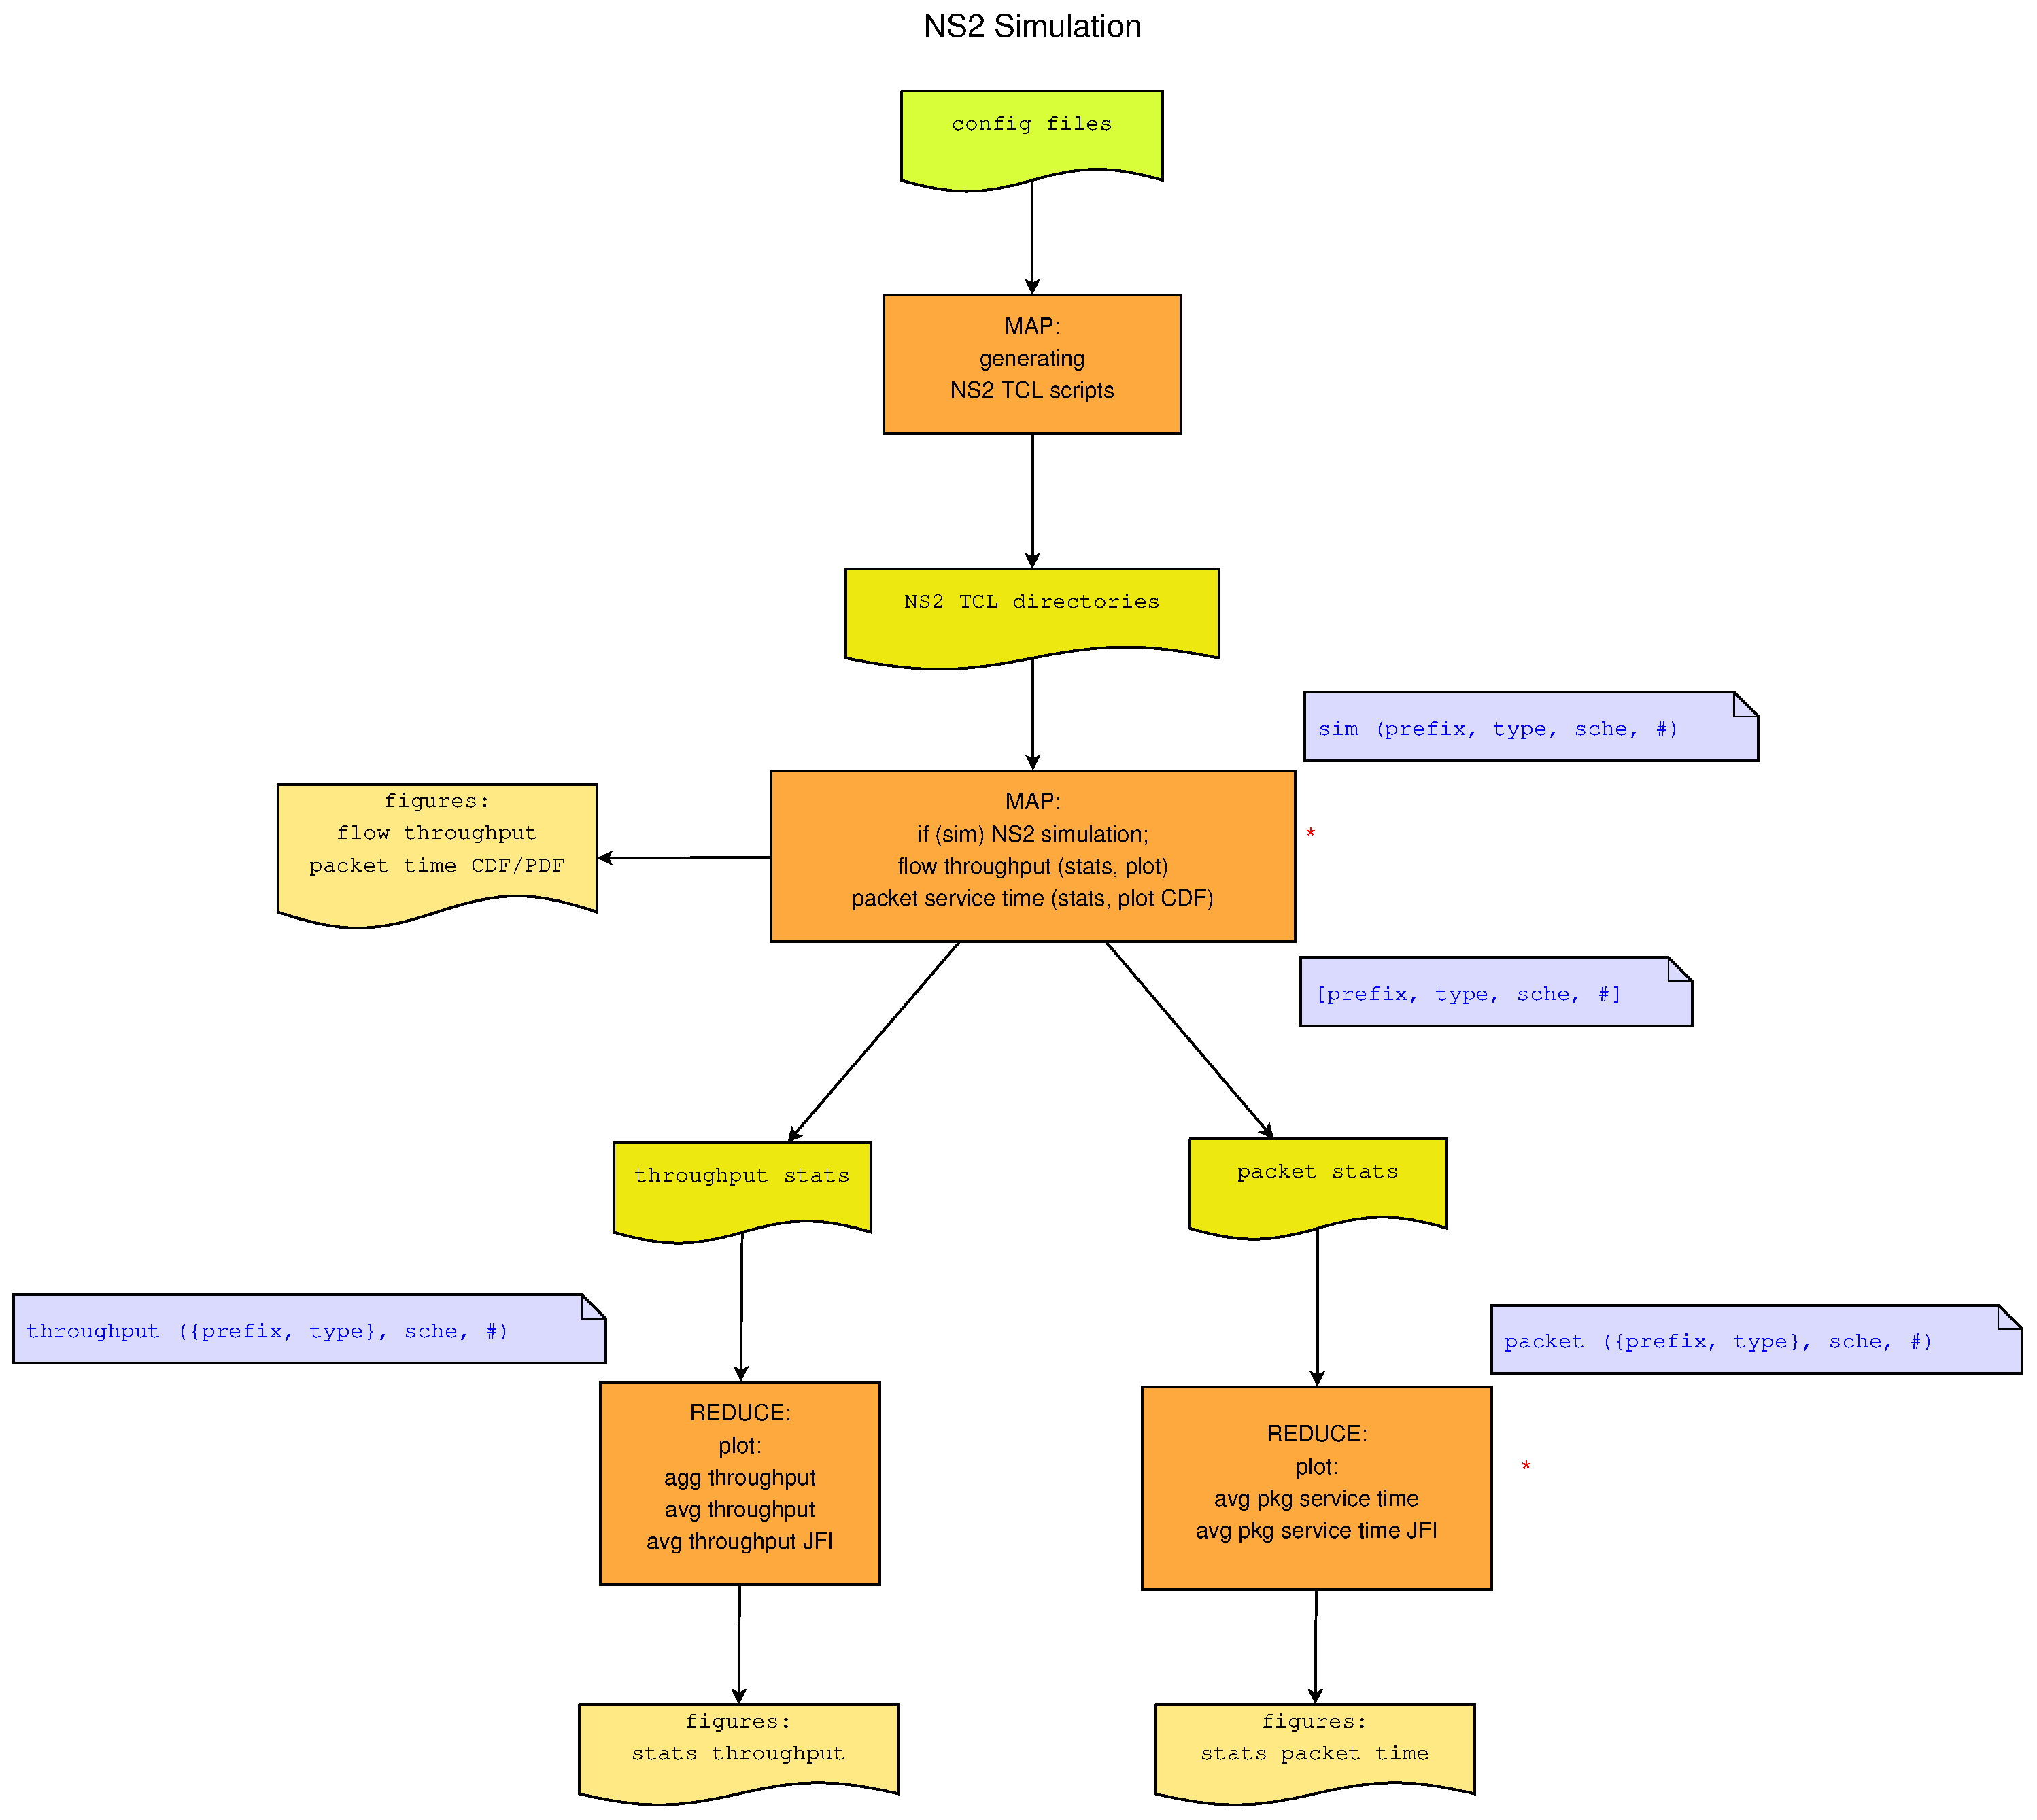
\includegraphics[width=0.9\textwidth]{flowchart-mr-ns2sim}
  \caption{The system.
    The text in \fcolorbox{black}{vidtransoriginfile}{this color} is the original input file.
    The text in \fcolorbox{black}{vidtranstmpfile}{this color} is the temp file.
    The text in \fcolorbox{black}{vidtransfinalfile}{this color} is the final output file.
    The text in \fcolorbox{black}{vidtransprocess}{this color} is process block.
    The text in \fcolorbox{black}{vidtransfuncio}{\textcolor[HTML]{0000FF}{this color}} is the input/output of one process block.
The process blocks signed by a \textcolor[HTML]{FF0000}{*} are the blocks cost most of the processing time.
  }\label{fig:system}
\end{figure}

The packet delay time processing includes:
\begin{itemize}
  \item (Mgn) filter out CMTS management packets and stats
  \item (DS) filter out CMTS--CM flow and stats
  \item (US) filter out CM-CMTS flow and stats
  \item Plot DS CDF/PDF
  \item Plot Managment CDF/PDF
\end{itemize}


\section{Low Level Design}

\subsection{main}


\subsubsection{Interface of the generating configurations}

Use the streaming mode of Map-Reduce.

The input should be the config file list.

\begin{itemize}
  \item \textbf{Map}
Function: generate directories and move and modify TCL scripts for the test.


Input parameters:
\begin{lstlisting}[language=bash]
<command> <config_file>
# config "/path/to/config.sh"
# config "/path/to/config-jjmbase.sh"
\end{lstlisting}


Output:
\begin{lstlisting}[language=bash]
<command> <config_file> <prefix> <type> <scheduler> <number_of_node>
sim <config_file> <prefix> <type> <scheduler> <number_of_node>
# sim "config-xxx.sh" "jjmbase"  "tcp" "PF" 24
\end{lstlisting}

There should exist the directory contains the TCL scripts and data files for the simulation.

\end{itemize}



\subsubsection{Interface of simulation}

This stage will run the simulation base on each directory configuration,
and also generate the related throughput figures.

\begin{itemize}
  \item \textbf{map}
Function: run the simulations.


Input parameters:
\begin{lstlisting}[language=bash]
<command> <config_file> <prefix> <type> <scheduler> <number_of_node>
sim <config_file> <prefix> <type> <scheduler> <number_of_node>
# sim "config-xx.sh" "jjmbase"  "tcp" "PF" 24
\end{lstlisting}


Output:
\begin{lstlisting}[language=bash]
<command> <config_file> <prefix> <type> <flow_type> <scheduler> <number_of_node>
throughput <config_file> <prefix> <type> <flow_type> <scheduler> <number_of_node>
packet <config_file> <prefix> <type> <flow_type> <scheduler> <number_of_node>
# throughput "config-xx.sh" "jjmbase"  "tcp" "tcp" "PF" 24
# packet "config-xx.sh" "jjmbase"  "tcp+has" "tcp" "PF" 24
\end{lstlisting}

The routine should run ns2 and process stats, figures of throughput/packet.




  \item \textbf{reduce}
Function: plot JFI figures


Input: (all of the columns are keys)
\begin{lstlisting}[language=bash]
<command> <config_file> <prefix> <type> <flow_type> <scheduler> <number_of_node>
throughput <config_file> <prefix> <type> <flow_type> <scheduler> <number_of_node>
packet <config_file> <prefix> <type> <flow_type> <scheduler> <number_of_node>
# throughput "config-xx.sh" "jjmbase"  "tcp" "tcp" "PF" 24
# packet "config-xx.sh" "jjmbase"  "tcp+has" "tcp" "PF" 24
\end{lstlisting}

Output: figures

\end{itemize}





\subsection{utils}

There're three types of environment be supported by the software,
which are single host bash, hadoop, and myhadoop.

In hadoop environment, the system will need HDFS to store both the data and executable for all of nodes involved.
\begin{itemize}
  \item executable: such as ns2 C++ binary and its support files
  \item data: config files and TCL scripts for the specific simulation
\end{itemize}
Once a node start to run the simulation, the map-reduce script should load the binary files from HDFS to local host first,
then read a global config file for environment settings,
and read a config file for that simulation to continue simulation.

While in myhadoop case, the data and executable are not necessary to be stored in HDFS since there's share file system for the HPC.
But the user should also be warned because some type of network file system (NFS) will downgrade the simulation speed if the simulator write the data to the NFS directly.
One of the trade-off is to copy the config files from the NFS to a directory of local disks and run the simulator on that directory and copy the data back to the NFS after finishing the simulation.

To overcome all of these challenges mentioned above,
we integrate the following functions in the software:
\begin{itemize}
  \item An abstract interface for the file system: it supports copy files, move files, print files on the standard output, find files etc. So that the software can support local files and HDFS files in a restricted computing environment (we're not system administrator and can't install various file system driver by ourselves.).
  \item use local disks to store data temporally: to speed up the simulation.
\end{itemize}

\begin{figure}\centering
  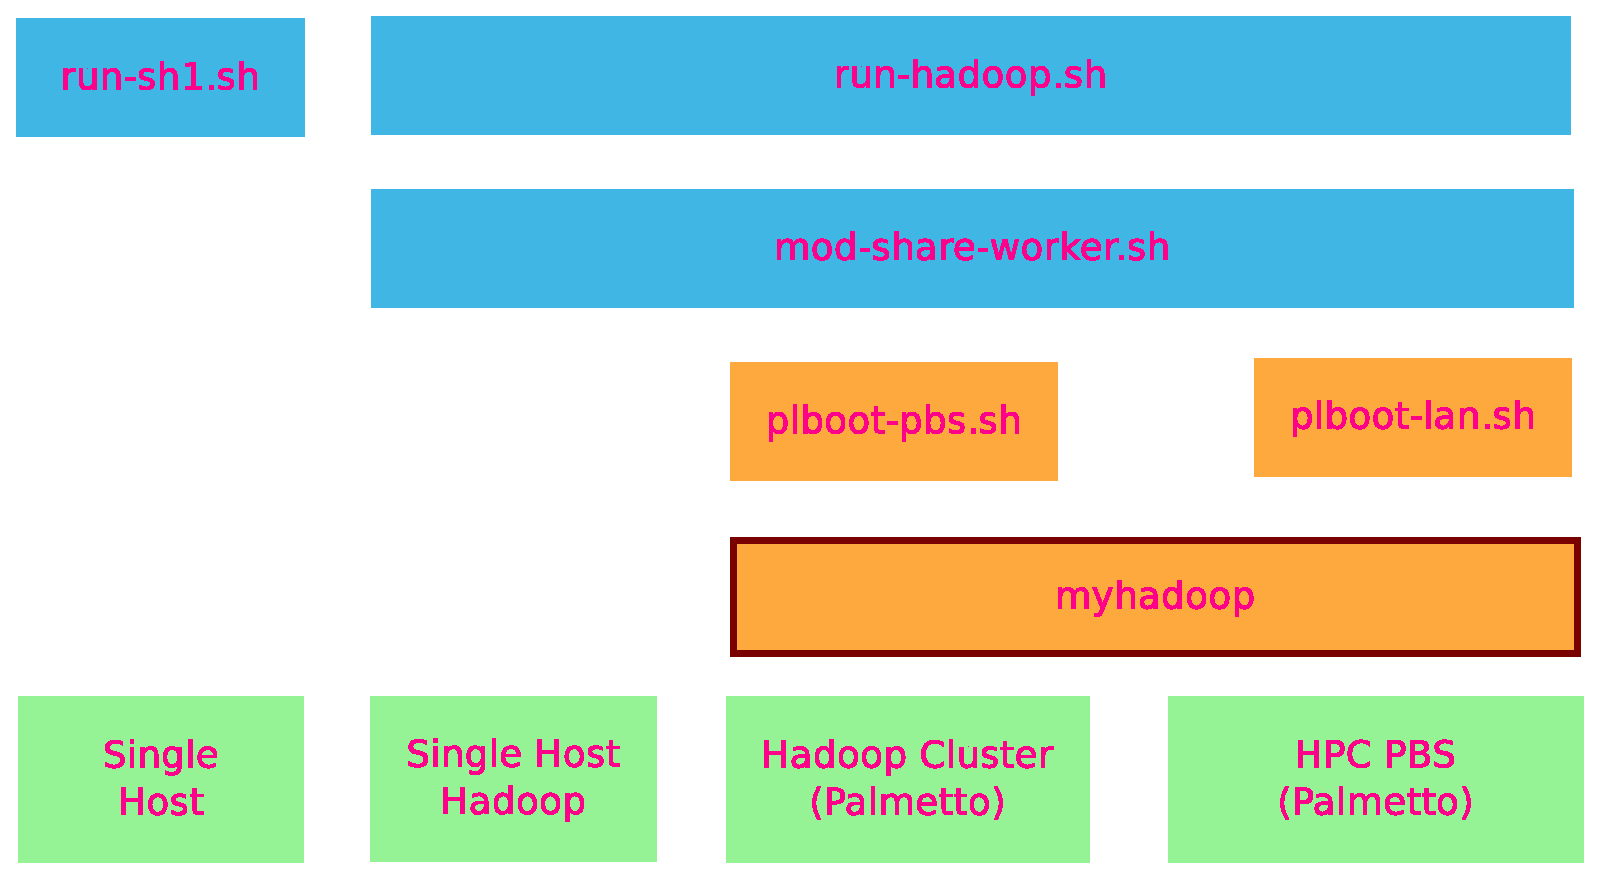
\includegraphics[width=0.9\textwidth]{mrnative-stack}
  \caption{The stack of the mrnative}\label{fig:mrnativestack}
\end{figure}

We have following program entrances for various execution environments:

\begin{itemize}
  \item \texttt{run-sh1.sh}, run in a single host, to test the basic functions of the software;


    It will call following scripts
    \begin{itemize}
      \item \texttt{e1map.sh}
      \item \texttt{e2map.sh}
      \item \texttt{e2red.sh}
      \item \texttt{e3map.sh}
    \end{itemize}
  \item \texttt{run-hadoop.sh}, setup basic Hadoop environment, copy executable and data to HDFS, call \texttt{mod-share-worker.sh};
    \begin{itemize}
      \item \texttt{mod-share-worker.sh}, the hadoop main script, it will submit various map-reduce tasks for the simulation and data processing;
        \begin{itemize}
          \item \texttt{e1map.sh}
          \item \texttt{e2map.sh}
          \item \texttt{e2red.sh}
          \item \texttt{e3map.sh}
        \end{itemize}
    \end{itemize}

  \item \texttt{run-hadooppbs.sh}, get available HPC resources, setup basic resources info for Hadoop (cores, memory etc.), submit \texttt{mod-hadooppbs-jobmain.sh} to the PBS;

    \begin{itemize}
      \item \texttt{mod-hadooppbs-jobmain.sh}, setup myHadoop environment;

        It setup myHadoop, start Hadoop over the nodes in HPC,

        and call \texttt{mod-share-worker.sh}:
        \begin{itemize}
          \item \texttt{mod-share-worker.sh}, the hadoop main script, it will submit various map-reduce tasks for the simulation and data processing;

          This script can runs in either Hadoop or myHadoop environment, and should using the environment variables from the setting scripts (\texttt{mod-hadooppbs-jobmain.sh} or \texttt{run-hadoop.sh})

          It also sets following variables:
            \begin{itemize}
              \item \texttt{EXEC\_HADOOP} \texttt{hadoop} command
              \item \texttt{HDJAR} find the \texttt{hadoop-streaming.jar}
            \end{itemize}


          It will call following scripts for map-reduce tasks:
            \begin{itemize}
              \item \texttt{e1map.sh}:

                1. \texttt{DN\_TOP} is the path to the scripts, to find the global config file \texttt{mrsystem.conf}; the \texttt{lib/libxxx.sh} and other files don't need be used since it is integrated in the \texttt{tempe1map.sh} by \texttt{mod-share-worker.sh};

                2. \texttt{HDFF\_DN\_SCRATCH} is the path that the program can store temporary data, it may be changed by the \texttt{e1map.sh} at the begin according to the computing environment limitations.

              \item \texttt{e2map.sh}
              \item \texttt{e2red.sh}
              \item \texttt{e3map.sh}
            \end{itemize}
        \end{itemize}

    \end{itemize}

\end{itemize}



The scripts such as \texttt{e1map.sh}, \texttt{e2map.sh}, \texttt{e2red.sh}, \texttt{e3map.sh} etc,
are executed in hadoop environment, so it should use the file system abstract interface when accessing file system.
The other scripts may use it for convenience.



The global variables (switches) in \texttt{mrsystem.conf}:
\begin{itemize}
  \item \texttt{HDFF\_DN\_SCRATCH}, a suggested local path to store temporary data;

  \item \texttt{HDFF\_DN\_OUTPUT}, the path that the results will be stored;
\end{itemize}



\subsection{Performance}


run in a single host with bash:

\begin{lstlisting}[language=bash]
config:
    HDFF_NUM_CLONE=4
    OPTIONS_FFM_GLOBAL=
Cost time: total=139 seconds
    stage1=10(m=10,r=0) seconds
    stage2=77(m=65,r=12) seconds
    stage3=(m=52,r=0) seconds
\end{lstlisting}


run in a single host hadoop:
\begin{lstlisting}[language=bash]
Cost time: total=2926,stage1=498,stage2=1697,stage3=731, seconds
\end{lstlisting}



